\documentclass[../summary.tex]{subfiles}

\begin{document}
	
\section{Climate}
\subsection{Introduction}
\subsubsection{Climate challenges}

The \textbf{Holocene} is a very stable period, started around 9000 years before Christ. This stable climate period was very good for society and agriculture to develop.\\
\\
\textbf{Oil} gets created when animals in the sea die, fall to the ground, are compacted and finally translate to oil.\\
\\
\textbf{Coal} get created when vegetation that grows on the surface dies, gets compacted first to peat and then under heat and pressure, gets further compacted to coal.\\
\\
Due to the warming - which is nowadays \textbf{1.2 degrees} Celsius compared to pre-industrial situations – extreme weather is exacerbated.\\
\\
There is an \textbf{impact on 3 systems}:
\begin{itemize}
	\setlength\itemsep{0.1em}
	\item Physical System (Glaciers, Snow, Sea Level, Precipitation)
	\item Biological System (Wildfires, Terrestrial Ecosystem, Marine Ecosystem)
	\item Human and Managed System (Food Production, Economical Systems)
\end{itemize}
\ \\
There are \textbf{2 big challenges}:
\begin{itemize}
	\item \textbf{Climate mitigation}, which means reducing climate change by reducing greenhouse gases in the atmosphere. Can be done in 2 ways: reduce the fossil fuels that are used and enhancing the sinks - the systems that capture carbon.
	\item \textbf{Climate adaptation}, society has to adapt to a changing climate because climate change is already there and will only continue to get worse.
\end{itemize}
\ \\

\subsection{Climate trends and causes}
\subsubsection{Climate change on geological timescales}

One of the best record to view the climate change over the last million years is the \textbf{Antarctic ice sheet}.\\
\\
Very old ice from e.g. 8000 years ago can be taken from the bottom of the Antarctic ice sheet up to the surface. Isotopic analysis of these samples allows the derivation of past temperatures, revealing variations of more than \textbf{12 degrees Celsius} across multiple glacial cycles in Antarctica. \\
\\
These climatic shifts are also evident in the landscape as glacial cycles caused ice caps to move southward toward the equator, leaving behind features like end moraines,  which is a small hill in the landscape. These get formed during a period where there was a lot of ice, which is called the Saalien. Interglacial periods, like the last one 125,000 years ago, were characterized by higher temperatures and sea levels, leading flooded land. 
\newpage
\subsubsection{Causes of climate change}

Throughout Earth's history, temperature fluctuations have occurred due to various factors. These include:
\begin{itemize}
	\item   Eccentricity e.g. changes in the Earth's orbit around the sun. \\
	(elliptical $\leftrightarrow$ circular)
	\item Obliquity e.g. axial tilt (more straight $\leftrightarrow$ more right) \ref{fig:obliquity}
	\item  Precession
\end{itemize}

\begin{figure}[h]
	\centering
	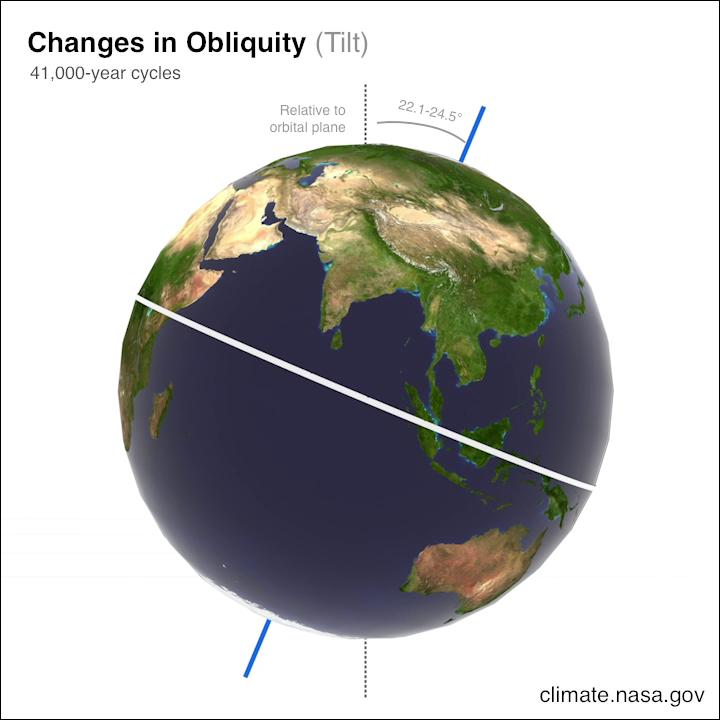
\includegraphics[width=0.5\linewidth]{images/obliquity_with_border}
	\caption[]{Obliquity of the Earth}
	\label{fig:obliquity}
\end{figure}
\ \\
Obliquity is very important, because it affects the distribution of sunlight and the size of ice caps. When the axis is more titled, summers are very hot and winters are very cold. This results in a positive feedback loop, which in this case is called the \textbf{albedo feedback}. This means that when it gets warmer, the size of the ice caps will decrease. Because of this, there will be less reflection of the sunlight, so it gets even warmer.\\
\\
Plate movements, volcanic eruptions, and solar activity e.g. radiation also influence climate.\\
\\
However, the recent climate change observed since industrialization is primarily caused by human activities, particularly the emission of greenhouse gases from burning fossil fuels. These gases contribute to the warming on Earth.\\
\\
During the burning of fossil fuel, tiny particles are emitted in the atmosphere, which reflect the solar radiation.  So they have a small compensating cooling effect on the earth.\\
\\
Feedback processes further intensify these effects, such as the already visible reduction in the Arctic sea ice, which leads to less reflection of sunlight by the ice
and leads to an additional warming of the climate system.
\newpage
\subsubsection{CO$_2$ Levels}

Since the emergence of Homo sapiens about 300,000 years before present, the variation of CO$_2$  has been between 180 and 280 parts per million volume. Today, it's 416 parts per million volume. This is almost 40\% higher. These high CO$_2$  values have been the most important cause of the warming of the Earth that we have seen since industrialization.

\begin{figure}[h]
	\centering
	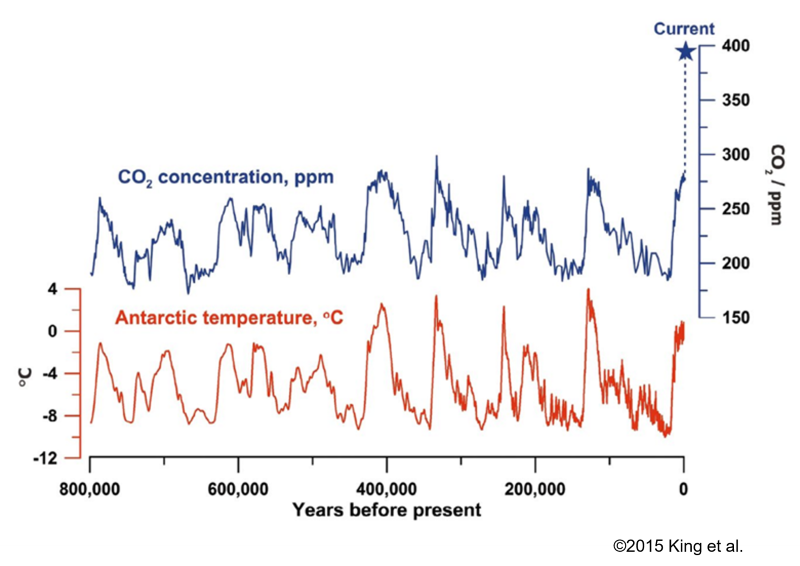
\includegraphics[width=0.7\linewidth]{images/Carbon_and_temperature_800k}
	\caption{CO$_2$ and temperature levels over the last 800,000 years before present}
	\label{fig:carbonandtemperature}
\end{figure}

\subsubsection{Humans caused climate change}

There are five lines of evidence that confirm that human-emitted greenhouse gases are responsible for global warming since industrialization:

\begin{itemize}
	\item \textbf{Global Carbon Budget}: Analysis of carbon emissions from burning fossil fuels and cement production, compared to emissions from land-use changes, shows that human activities emit the most. A large part of this emission is captured by the ocean and the land. Would this not be the case, then the atmospheric CO2 concentrations would be doubled.
	
	\begin{figure}[H]
		\centering
		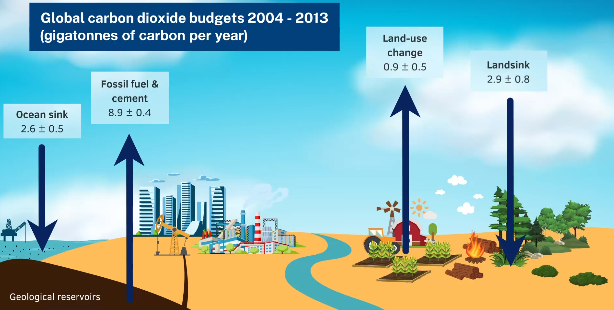
\includegraphics[width=0.7\linewidth]{images/carbon_budget}
		\caption{Global carbon budget}
		\label{fig:carbonbudget}
	\end{figure}
	
	\item \textbf{Isotopic Ratio}: The isotopic ratio of carbon in the atmosphere decreases over time due to the burning of fossil fuels, which releases carbon with a specific isotopic signature. This isotopic ratio is roughly the same as for plants and is about 2\% lower than that of the atmosphere. 
	
	\begin{figure}[H]
		\centering
		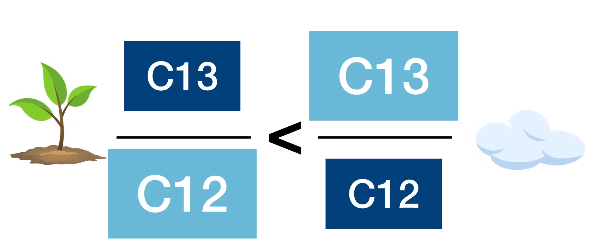
\includegraphics[width=0.7\linewidth]{images/isotopic_ratio}
		\caption{Isotopic ratio of plants and the atmosphere}
		\label{fig:isotopicratio}
	\end{figure}
	
	
	\item \textbf{Physical Mechanism}: The sun emits solar radiation that is partly reflected back to space. The Earth and the atmosphere emit infrared radiation.
	This infrared radiation is absorbed into gases in the atmosphere and also partly by clouds and re-emitted back to the surface. So this infrared radiation cannot escape to space. And this then causes a warming of the earth system.
	
	\item \textbf{Climate Models}: Climate models, when run with only greenhouse gases that have been occuring in the atmosphere, show a larger temperature increase than observed, indicating that greenhouse gases  have a larger effect on temperature than observed. Aerosols,which are tiny particals formed by fossil fuel burning that reflect solar radiation, provide a partial cooling effect.
	
	\begin{figure}[H]
		\centering
		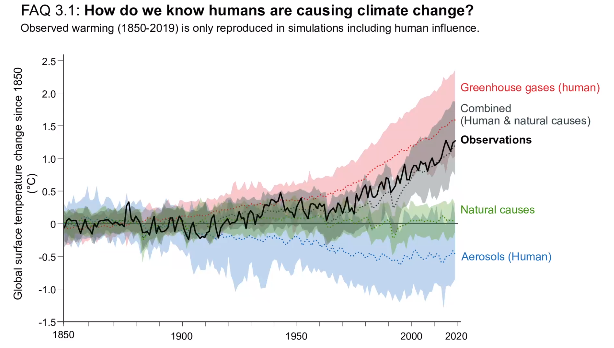
\includegraphics[width=0.8\linewidth]{images/model}
		\caption{Climate model}
		\label{fig:model}
	\end{figure}
	
	
	\item \textbf{Radiative Forcing}: Radiative forcing is what happens when the amount of energy that enters the Earth's atmosphere is different from what leaves it.
\end{itemize}

\newpage

\subsubsection{Radiative forcing}

The Earth and atmosphere exchanges energy with space through radiation, with incoming solar radiation (342 W/m²), of which 31\% gets reflected (170 W/m²) and 235 W/m² gets absorbed, and outgoing infrared radiation (235 W/m²) balancing each other out.\\
\\
Radiative forcing is the disturbance in this balance due to external factors, such as increased greenhouse gases. When radiative forcing occurs, an imbalance leads to warming (more incoming radiation) or cooling (more outgoing radiation) until equilibrium is re-established.\\
\\
Carbon dioxide (CO2) is the dominant contributor to radiative forcing, with methane also playing a significant role. Other greenhouse gases, such as ozone and nitrous oxide, contribute but to a lesser extent than CO2.\\
\\
Aerosols, emitted from fossil fuel burning, result in negative radiative forcing by reflecting solar radiation. Natural variations, like volcanic eruptions, also have short-term impacts on radiative forcing.\\
\\
Over time (since 1750), CO2 has shown the largest increase in radiative forcing, making it a central driver of climate change. The radiative forcing of greenhouse gases combined is larger than the total radiative forcing, emphasizing their collective impact. Uncertainties exist in radiative forcing estimates, with larger uncertainties associated with aerosols than greenhouse gases.

\subsection{Climate targets and pathways}
\subsubsection{International agreements}
The Paris Agreement, a pivotal moment in climate negotiations, aims to stabilize greenhouse gas concentrations. It sets a goal to limit global warming to well below 2 degrees Celsius, preferably 1.5 degrees Celsius compared to pre-industrial levels. These targets are based on scientific research and risk assessments by the Intergovernmental Panel on Climate Change (IPCC).\\
\\
Burning ember diagrams, created by IPCC experts, categorize concerns into five reasons for concern:
\begin{itemize}
	\item Systems with restricted range (e.g., coral reefs, Arctic, indigenous people) face increasing risks with higher warming.
	\item Extremes like heatwaves, heavy rains, and wildfires already show moderate risk and increase with more warming.
	\item Impacts disproportionately affecting certain groups see risks rise with warming.
	\item Global monetary damage risks, including global-scale degradation and ecosystem loss, increase at higher warming levels.
	\item Large, abrupt, and sometimes irreversible changes (tipping points) also pose greater risks with elevated warming. For example the disintegration of the Antarctic ice sheet.
\end{itemize}

\begin{figure}[H]
	\centering
	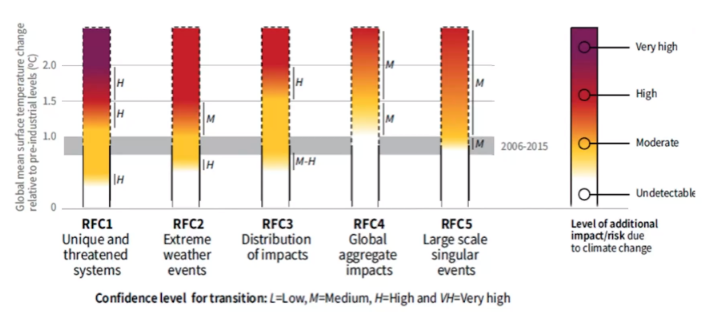
\includegraphics[width=0.6\linewidth]{images/impacts_and_risks}
	\caption{Impacts and risks with the Reasons for Concern (RFCs)}
	\label{fig:impactsandrisks}
\end{figure}
\ \\
The 1.5 and 2 degrees Celsius targets of the Paris Agreement were chosen based on this risk assessment. The burning ember diagrams demonstrate that exceeding these targets would significantly increase the risks of adverse climate impacts.\\
\\
The burning ember diagrams also show that risks increase with higher warming levels across natural, managed, and human systems. Even at a global warming of 1 degree Celsius, vulnerable regions may experience high climate risks.\\
\\
The global scientific community and the IPCC have played a key role in underpinning policy decisions. Greenhouse gas emissions are identified as the primary cause of warming, and adhering to the Paris Agreement targets is crucial to prevent the worst impacts on the climate system and society.

\subsubsection{Carbon budget}

To be able to set emission reduction targets the concept of the carbon budget was introduced. The carbon budget is the amount of carbon that can be emitted over a period of time before a certain temperature target is reached.\\
\\
It's important to note that every ton of CO2 contributes to warming, regardless of when it's emitted. This means the carbon budget includes emissions from the beginning of industrialization to the present day, known as the historical carbon budget. The portion of the budget that can still be utilized, which currently is 20\%, is referred to as the remaining carbon budget.\\
\\
The relationship between CO2 emissions and global warming is nearly linear, meaning double the emissions lead to double the warming. However, there is some uncertainty in this relationship. To increase our confidence in achieving temperature targets, we choose a carbon budget that provides a 66\% probability of staying within the goals set by the Paris Agreement.\\
\\
Other greenhouse gases are considered using global warming potential (GWP), measuring their impact compared to CO2 over 100 years. For example, methane has a GWP 23 times that of CO2, making it more potent, while nitrous oxide (N2O) is 296 times as powerful. Certain hydrofluorocarbons have a GWP of up to 12,000 but are emitted in smaller quantities than CO2.

\subsubsection{Emission pathways}

The concept of the carbon budget provides a quantitative approach to achieve global temperature targets, such as the Paris Agreement's goals. Different emission reduction pathways exist, some with early strong cuts and others with later but steep reductions, relying on unproven negative emissions technology.\\
\\
The key is to reduce fossil fuel use, while land management (like planting trees) and carbon capture and storage can also help. However, carbon capture and storage has limitations and challenges.\\
\\
Emission Gap reports show that while policies are reducing emissions, there's still a significant gap between what countries promise (Nationally Determined Contributions) and what's needed to meet the Paris Agreement's targets.\\
\\
Without policies, global warming could reach catastrophic levels (4.1-4.8°C). Current policies are insufficient, targeting around 2.9°C, and even the unconditional pledges aim for a 2.6°C warming level, emphasizing the need for more ambitious and effective climate action.
\newpage
\subsection{Climate mitigation}
\subsubsection{Collective and individual action}

To combat the climate crisis, the first step is to educate yourself about climate solutions. The Drawdown project provides valuable information on effective climate solutions across various sectors. Drawdown is the point in the future when levels of greenhouse gases in the atmosphere stop climbing and start to steadily decline. Drawdown estimates the reduction or sequestration of emissions from 2020 to 2050 based on climate targets, such as the two-degree target.\\
\\
Some of the top climate solutions from different sectors include:

\begin{itemize}
	\item \textbf{Reducing Food Waste}: A significant reduction in food waste can cut 88.5 gigaton CO2 equivalents, equivalent to 2.2 years of current emissions.
	\item \textbf{Plant-Rich Diets}: Shifting toward plant-based diets or reducing meat and dairy consumption helps combat the climate crisis.
	\item \textbf{Family Planning and Education}: Promoting family planning and education can contribute to reducing CO2 emissions.
	\item \textbf{Refrigerant Management and Alternative Refrigerants}: Managing refrigerants and transitioning to alternatives is crucial due to the high global warming potential of some refrigerants.
	\item \textbf{Tropical Forest Restoration}: Restoring tropical forests increases carbon sequestration.
	\item \textbf{Transition to Renewable Energy}: Adoption of renewable energy sources, including onshore wind turbines, utility-scale solar photovoltaics, and distributed solar photovoltaics, plays a vital role.
	\item \textbf{Clean Cooking}: Improving cooking methods and technologies in households reduces emissions.
\end{itemize}
\ \\
There's no single "silver bullet" solution, and a combination of multiple strategies and sectoral transformations is necessary to address the climate crisis effectively.

\subsubsection{Individual action}

There are several ways you can contribute to fighting climate change:

\begin{itemize}
	\item \textbf{Use Your Democratic Right}: Stay informed about political parties and their climate policies. Participate in marches and climate activism to exert political pressure.
	\item \textbf{Reduce Your Carbon Footprint}: Start by educating yourself on effective solutions and tracking your carbon footprint. Reduce emissions through changes in energy use, mobility (such as walking, cycling, and using public transport), and limiting air travel. Be mindful of your diet as food production contributes significantly to emissions. Beef, lamb and cheese have the highest carbon footprint..
	\item \textbf{Consider Planet-Friendly Investments}: Opt out of funds investing in fossil fuels and explore ethical banks and investment opportunities.
	\item \textbf{Support Upscaling the Transition}: Share your eco-friendly choices with others through in-person discussions or social media. Join local or global climate movements and consider contributing to climate litigation to set legal precedents for climate change mitigation.
\end{itemize}
\ \\
Every action, no matter how small it may seem, matters in the fight against the climate crisis. Celebrate your contributions and explore the ways that best suit your lifestyle and values.
\newpage

\subsection{What can we expect for the future?}
\subsubsection{Climate scenario's}

The future of our climate depends on the actions we take to reduce greenhouse gas emissions. Climate scenarios are generated using complex computer models known as General Circulation Models (GCMs) and Representative Concentration Pathways (RCPs). RCPs represent different greenhouse gas concentration trajectories based on their radiative forcing. Here are some key points:

\begin{itemize}
	\item \textbf{Paris Agreement Targets}: The Paris Agreement aims to limit global warming to well below 2 degrees Celsius compared to pre-industrial levels, with an aspiration to limit it to 1.5 degrees Celsius. The target closest to the Paris Agreement is reflected in RCP 2.6, with a global warming range of 1.3 to 2.4 degrees Celsius by the end of the century.
	\item \textbf{Other RCP Scenarios}: RCP 8.5, representing a radiative forcing of 8.5 watts per square meter, doesn't align with the Paris Agreement and reflects a high level of emissions. Other scenarios like RCP 4.5 and RCP 6 also fall outside the Paris Agreement targets.
	\item \textbf{Regional Variation}: The intensity of warming varies by region, with polar regions experiencing more significant warming. This has implications for polar ice caps and sea ice. On the other hand, the ocean warms less because it has a large heat capacity. So it takes a lot more energy to warm.
	\item \textbf{Precipitation Changes}: Changes in precipitation are also region-specific. Wet regions are projected to get wetter, while dry regions may become drier. Extreme precipitation is expected to increase almost everywhere, with a more significant increase at higher global warming levels.
	\item \textbf{Impacts on Extreme Events}: Various extreme events, such as heatwaves, heavy rainfall, droughts, wildfires, and coastal flooding, are expected to become more severe with higher global warming levels. The larger the warming level, the more pronounced these impacts will be.
\end{itemize}
\ \\
Overall, the magnitude of global warming, driven by greenhouse gas emissions, determines the extent of temperature and precipitation changes, as well as the intensity of extreme events. It's crucial to reduce emissions and align with the Paris Agreement to mitigate these impacts and maintain a manageable world.\\
\\
Figure \ref{fig:climaticrange} shows the impact of global warming on the climatic range of  different species.

\begin{figure}[H]
	\centering
	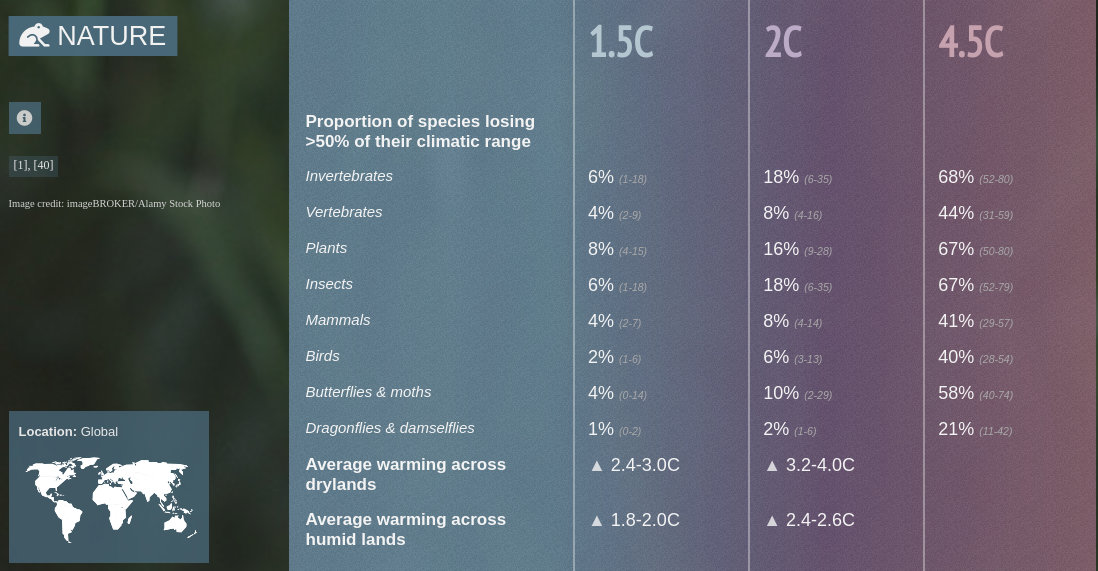
\includegraphics[width=0.8\linewidth]{../images/climatic_range}
	\caption{Reduction of climatic ranges of species at certain global warming levels}
	\label{fig:climaticrange}
\end{figure}

\subsubsection{Futures wheel}

The futures wheel is a method to make a \textbf{graphical visualization of direct and indirect future consequences of a particular change or development.} At the center of the wheel lies a circle describing the change. Then, events or consequences following directly from that development are positioned around it. Next, the (indirect) consequences of the direct consequences are positioned around the first level consequences, and so on.

\begin{figure}[H]
	\centering
	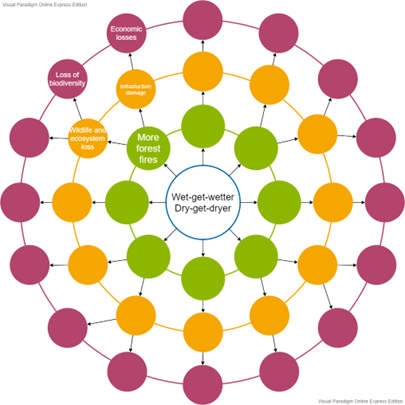
\includegraphics[width=0.45\linewidth]{../images/futures_wheel}
	\caption{Example of a futures wheel}
	\label{fig:futureswheel}
\end{figure}

\subsubsection{Sea level rise}

Sea-level rise is a significant concern associated with climate change. There are some contributors to Sea-Level Rise:

\begin{itemize}
	\item \textbf{Thermal expansion}: As the Earth's oceans warm due to climate change, seawater expands, contributing to sea-level rise.
	\item \textbf{Melting of glaciers and ice sheets}: The melting of glaciers or ice sheets on land also adds water to the oceans, further raising sea levels.
	\item \textbf{Change of land height}: The sea level can stay the same, but if there is a reduction of land height, the relative sea level can change at a certain location.

\end{itemize}
\ \\
The oceans have absorbed 90\% of the excess heat linked to climate change. But this means that the sea water has been expanding and the thermal expansion was the largest term of the sea level rise over the last century.\\
\\
Many glaciers around the world are retreating rapidly due to rising temperatures. This is particularly evident in regions like the Alps, where glaciers are receding, and only a few high-altitude ice fields remain. The extent of glacier ice remaining is sensitive to the level of global warming, with higher levels resulting in more significant losses.\\
\\
Both the Greenland and Antarctic ice sheets are experiencing mass loss. For Antarctica, the most significant reductions are observed in the West Antarctic ice sheet and the Pine Island Glacier region. The potential sea-level rise from these ice sheets is substantial, with Antarctica having the capacity to contribute up to 58 meters of sea-level rise and Greenland up to 7 meters.\\
\\
Currently, thermal expansion of the oceans (50\%) and glacier melt (25\%) are the two main contributors to sea-level rise. While the contributions from the polar ice sheets are currently smaller, they are expected to increase in the future.

\begin{figure}[H]
	\centering
	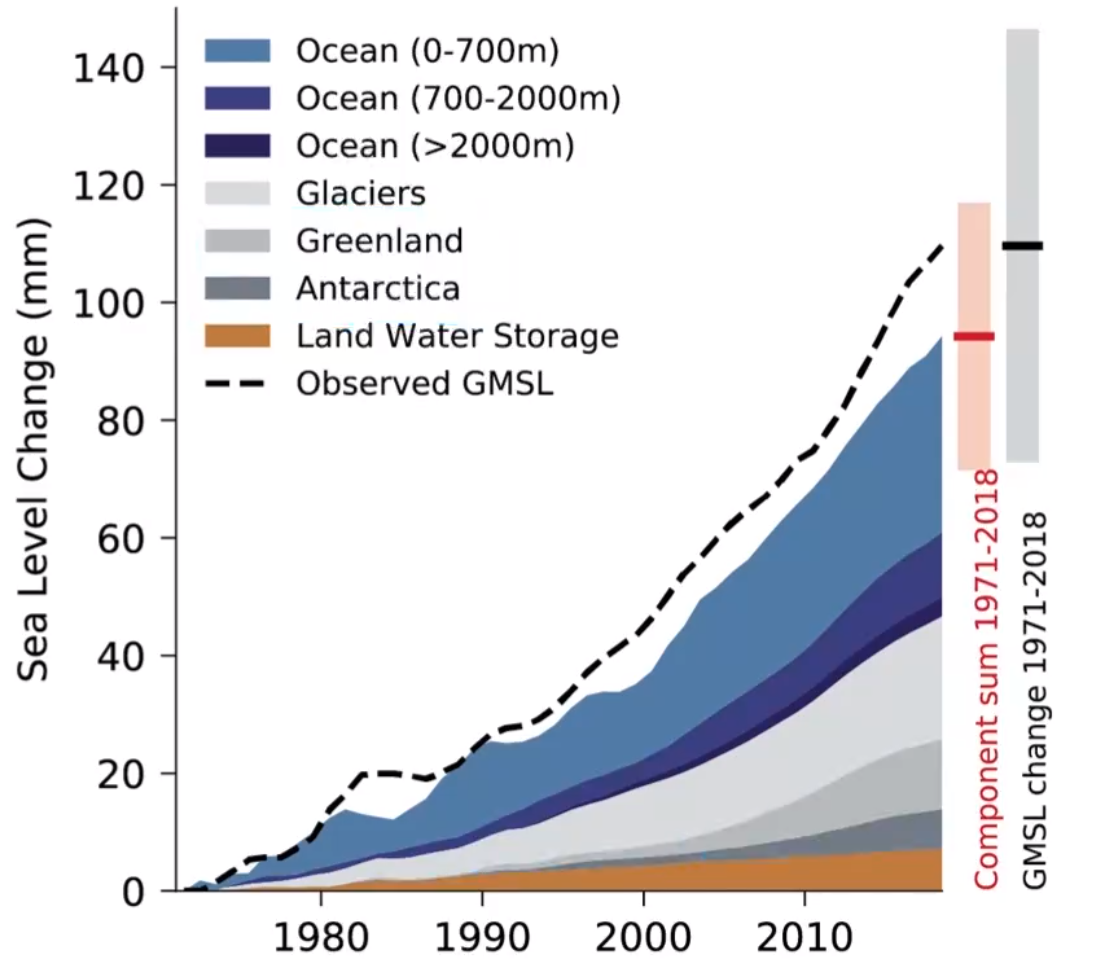
\includegraphics[width=0.57\linewidth]{../images/sea_level_rise}
	\caption{Sea level rise over time}
	\label{fig:sealevelrise}
\end{figure}
\ \\
There is a significant level of uncertainty regarding the behaviour of the Antarctic ice sheets. These ice sheets could be sensitive to disintegration, which may lead to more substantial sea-level rise than currently predicted.\\
\\
The level of future sea-level rise depends on global warming levels and emissions scenarios. Projections from the Intergovernmental Panel on Climate Change (IPCC) range from about 25 centimetres to approximately one meter of sea-level rise by the end of the century. The higher the emissions, the greater the potential for sea-level rise.

\begin{figure}[H]
	\centering
	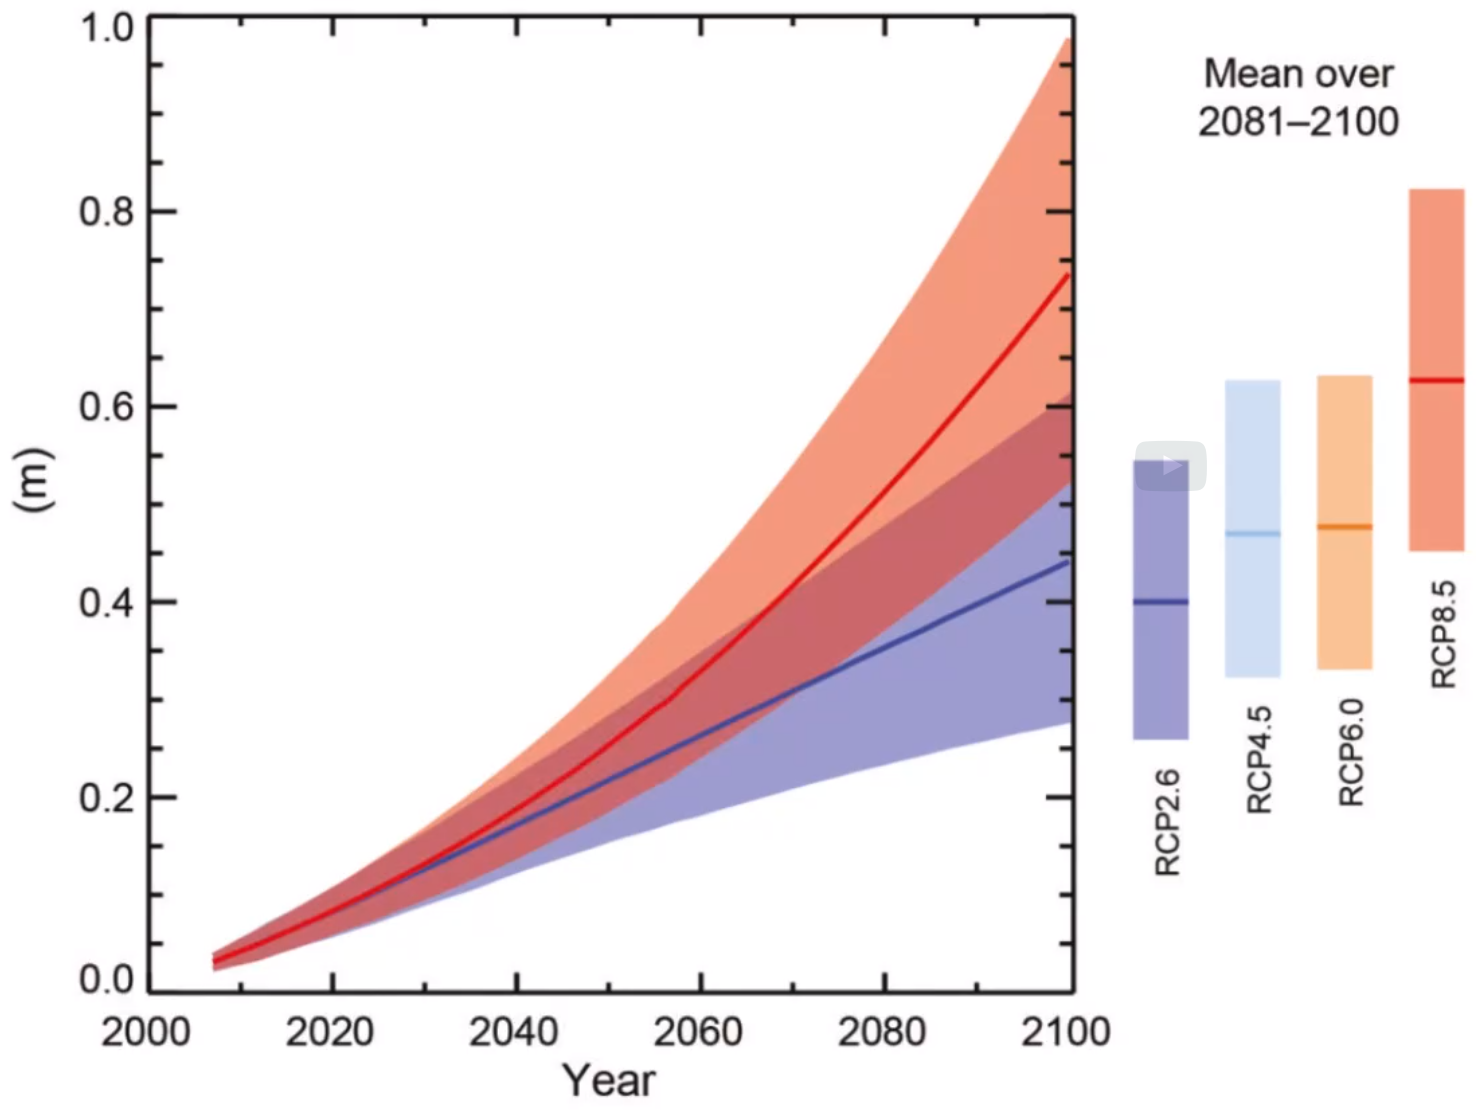
\includegraphics[width=0.6\linewidth]{../images/global_mean_sea_level_rise}
	\caption{Global mean sea level rise}
	\label{fig:globalmeansealevelrise}
\end{figure}
\ \\
Dealing with sea-level rise is a complex challenge. Even with significant efforts to reduce emissions, some sea-level rise is inevitable. The uncertainty associated with the Antarctic ice sheets adds complexity to future planning and adaptation efforts.\\
\\
Sea-level rise poses significant risks to coastal regions and low-lying countries. Burning ember diagrams are used to assess the risks associated with sea-level rise. These diagrams show that as sea level rises, the risks increase. Different coastal regions have varying levels of adaptation potential.

\begin{itemize}
	\item \textbf{Resource-Rich Coastal Cities}: Coastal cities with abundant resources have detectable risks due to sea-level rise, which can increase to a moderate to high risk with higher sea-level rise. These regions have some adaptation potential, but impacts are inevitable.
	\item \textbf{Urban Atolls and Islands}: Urban atolls and islands are highly vulnerable to sea-level rise, with very high risks. The adaptation potential is limited, and the risks remain even with sea-level rise of about 1 meter.
	\item \textbf{Large Tropical Agricultural Deltas}: Regions with large tropical agricultural deltas also face risks from sea-level rise, with some adaptation potential. However, higher sea levels still result in moderate to high risks.
	\item \textbf{Arctic Communities}: Arctic communities have a high risk of sea-level rise impacts. Some adaptation potential exists, but the risks cannot be fully mitigated.
\end{itemize}
\ \\
Flooding in coastal cities due to sea-level rise and storm surges results in significant economic costs. The annual flood costs for major cities are projected to reach billions by the middle of the century.\\
\\
By the middle of the century, over 570 low-lying coastal cities are expected to experience sea-level rise of at least half a meter. This will put more than 800 million people at risk from rising sea levels and storm surges.\\
\\
Addressing sea-level rise requires a combination of mitigation efforts to reduce emissions and limit global warming, as well as adaptation strategies to protect coastal regions. Both are essential to ensure the livability of our planet and to manage the risks associated with rising sea levels.


\end{document}